The record-to-record variability is one of the most important sources of uncertainty in fragility assessment. In the Direct Nonlinear Static Procedures implemented in the Risk Modellers Toolkit (see Section~\ref{subsec:direct-nsp}), this source of uncertainty is directly introduce in the fragility estimates, based on previous nonlinear analyses. In the Record-based Nonlinear Static Procedures (Section~\ref{subsec:record-nsp}) or in the Nonlinear Time History Analysis in Single Degree of Freedom Oscilators (Section~\ref{subsec:NLTHA_SDOF}), users have the possibility of introducing their own ground motion records. Each accelerogram needs to be stored in a \verb=csv= file (tabular format), as depicted in Table~\ref{table:gmr}. This file format uses two columns, in which the first one contains the time (in seconds) and the second the corresponding acceleration (in g).\\

\begin {table}[htb]
\caption{Example of a ground motion record.}
\label{table:gmr}
\begin{center}
  \begin{tabular}{ | c | c |}
  \hline
0.01 & 0.0211 \\ \hline
0.02 & 0.0292 \\ \hline
0.03 & 0.0338 \\ \hline
0.04 & 0.0274 \\ \hline
0.05 & 0.0233 \\ \hline
0.06 & 0.0286 \\ \hline
0.07 & 0.0292 \\ \hline
0.08 & 0.0337 \\ \hline
0.09 & 0.0297 \\ \hline
0.1 & 0.0286 \\ \hline
... & ...  \\ \hline
  \end{tabular}
\end{center}
\end{table}

In order to load a set of ground motion records into the Risk Modellers Toolkit, it is necessary to import the module \verb=utils=, and specify the location of the folder containing all of the ground motion records using the parameter \verb=gmrs_folder=. Then, the collection of records can be loaded using the following command:

\begin{Verbatim}[frame=single, commandchars=\\\{\}, samepage=true]
gmrs = utils.read_gmrs(gmrs_folder)
\end{Verbatim}

One the ground motion records have been loaded, it is possible to calculate and plot the acceleration and displacement response spectra. To do so, it is necessary to specify the minimum and maximum period of vibration to be used in the calculations, using the variables \verb=minT= and \verb=maxT=, respectively. Then, the following command must be used:

\begin{Verbatim}[frame=single, commandchars=\\\{\}, samepage=true]
minT = 0.1
maxT = 2
utils.plot_response_spectra(gmrs,minT,maxT)
\end{Verbatim}

This will generate three plots: 1) spectral acceleration (in g) versus period of vibration (in sec); 2) spectral displacement (in m) versus period of vibration (in sec); and spectral acceleration (in g) versus spectral displacement (in m). Figure \ref{fig:gmrs} illustrates the first two plots for a hundreds ground motion records.


\begin{figure}[!htbp]
\centering
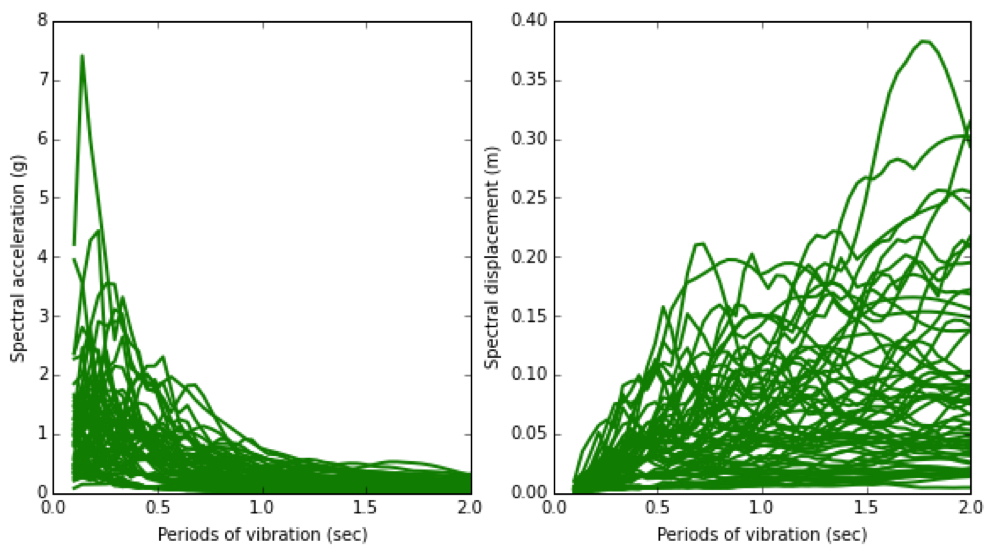
\includegraphics[width=12cm]{figures/gmrs.png}
\caption{Response spectra in terms of spectral acceleration versus period of vibration (left) and spectral displacement versus period of vibration (right).}
\label{fig:gmrs}
\end{figure}
